\chapter{Entorno Software}\label{cap:planificación}
Tal y como se menciona a lo largo de la memoria, el desarrollador debe de tener una estructura y un entorno de trabajo que garantice la correcta funcionalidad de todas las herramientas facilitadas para el desarrollo. 

Son diferentes las herramientas que se prepararán a lo largo de la memoria, todas las herramientas, funcionan bajo licencias de software libre, y son completamente gratuitas de utilizar. Dado que el entorno está orientado a el desarrollo de firmware para robot móviles, el entorno se encapsulará para que todo se ejecute sobre el sistema operativo Linux. El motivo por el que se ha elegido Linux como base de desarrollo es por ser el sistema operativo principal para el desarrollo de software, ya que está construido bajo licencias de software libre.

Para el desarrollo de 
\section{Linux}
\section{ROS}
\section{Entorno desarrollo Robot}

\subsection{Puesta a punto Coral TPU}

Con el objetivo de poder llevar a cabo la detección de objetos a tiempo real, se ha hecho uso de un acelerador gráfico USB, en concreto un dispositivo TPU (Tensor Procesor Unit) el cual se encargará de poder llevar a cabo el cálculo y procesado relacionado con la detección de objetos y la aplicación y procesado del modelo matemático.

Para poder llevar a cabo el procesamiento de las imágenes y el cálculo estructural de la red neuronal, se utilizan dispositivos a los que comúnmente se les denomina acelerador gráfico. Estos dispositivos se encargar de soportar el peso computacional correspondiente a los cálculos asociados a los modelos matemáticos. En este caso, el gran parte del peso del procesado recae sobre el modelo matemático y su procesado en CPU, es por ello, que para obtener unos mejores tiempos de respuesta y poder llevar a cabo un procesado en tiempo real y con una latencia baja se utilice una TPU.

\begin{figure}[h]
    \centering
    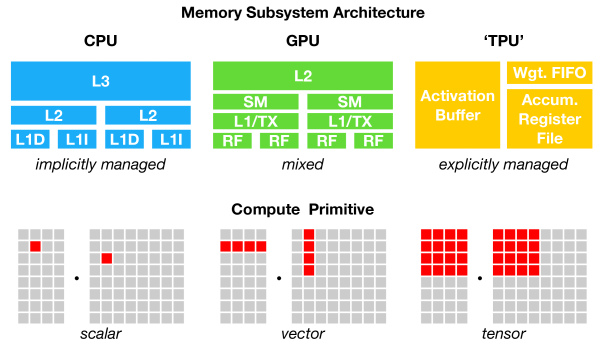
\includegraphics[scale=0.5]{fig/tpuVScpu.png}
    \caption{Comparativa CPU, GPU y TPU.}
    \label{fig:mesh1}
\end{figure}

Tal y como se puede observar en la figura XX, cada una de los diferentes tipos de procesadores destaca en un ámbito diferente y cada un o tiene su aplicaciones particular. En lo que atañe al proyecto, ya que la carga de trabajo con mayor peso recae sobre el modelo de inteligencia artificial, la mejor opción para poder ejecutar todos estos cálculos de la manera más eficiente es utilizar una TPU.

Las TPU son capaces de procesar la información de modelos matemáticos, como por ejemplo las redes neuronales, de 15 a 30 veces mas rápido que una GPU convencional, además de ser mas eficientes energéticamente debido a su bajo consumo. El inconveniente de estos dispositivos es la baja versatilidad a la hora de incluirlos en el proyecto. Para la aplicación deseada encaja perfectamente debido al tipo de procesado que realizará, el bajo coste económico y la fácil instalación del dispositivo en el sistema operativo gracias a su conexión USB 3.0. 

\begin{figure}[h]
    \centering
    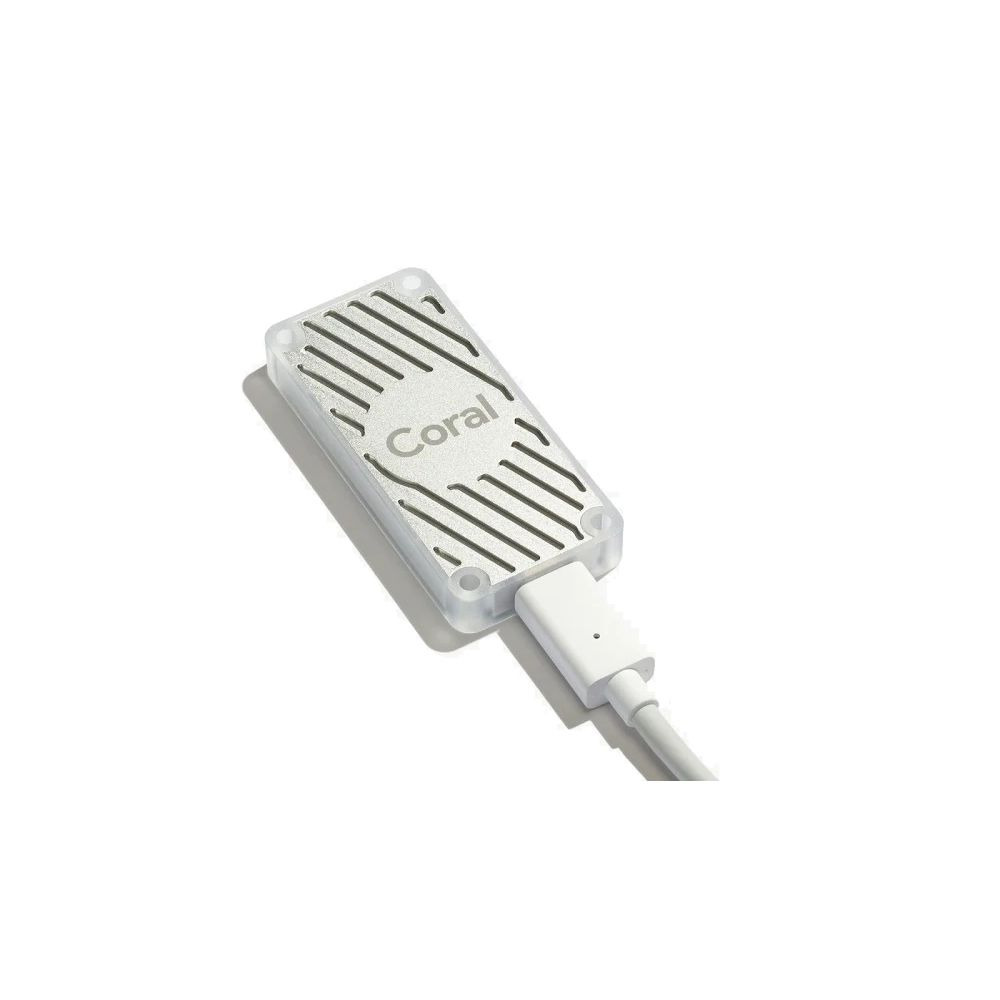
\includegraphics[scale=0.5]{fig/google_coral_usb_accelerator_1.jpg}
    \caption{Google Coral TPU USB Accelerator.}
    \label{fig:mesh1}
\end{figure}

Para poder poner en funcionamiento la TPU se deben de cumplir una serie de requisitos software para que el sistema operativo sea capaz de trabajar con el hardware. Es necesario instalar una serie de drivers para que se pueda establecer un entendimiento hardware-software y de esa forma poder realizar la mayor parte del procesado en este hardware.

Para poner a punto la Coral TPU y poder comprobar su correcto funcionamiento, el primero de los pasaos a seguir es instalar un gestor de paquetes para poder resolver todas las dependencias que se vayan necesitando a lo largo de la instalación y puesta a punto. En el caso de los proyectos, se ha instalado conda para poder gestionar entornos e instalar los diferentes paquetes para python que se van necesitando a lo largo de la puesta en marcha. 

\begin{figure}[h]
    \centering
    
\includegraphics[scale=0.5]{fig/python-conda.png}
    \caption{Gestor de paquetes y entornos Conda.}
    \label{fig:mesh1}
\end{figure}

Se ha de tener en cuenta la distribución y arquitectura que presentará el proyecto a la hora de poder instalar un paquete determinado ya que dependiendo de cada arquitectura, distribución y kernel de cada uno de los sistemoas operativos y harware que se esté utilizando se deberá de adaptar a un software y otro.

Para el caso del proyecto, se esta ejecutando todo el código sobre un linux, con una distribución basada en ubuntu server al que se le ha instalado un entorno gráfico. A la hora de instalar el gestor de paquetes Conda hay que tener en cuenta diversos factores diferenciales.

Primero debemos de conocer la arquitectura y la version del sistema operativo sobre el cual estamos ejecutando, para ello se pude abrir una ventana de comandos o terminal y ejecutar el siguiente comando: "uname -m".

\begin{figure}[h]
    \centering
    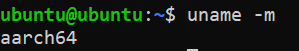
\includegraphics[scale=1.5]{fig/uname -r.PNG}
    \caption{Ejecución de comando "uname -r".}
    \label{fig:mesh1}
\end{figure}

Tal y como se puede observar en la figura XX, el comando uname -r nos muestra en la terminal el tipo de arquitectra sobre el que estamos trabajando. Como era de esperar, Raspberry trabaja con una CPU ARM, por lo cual el resultado de ejecutar el comando es "aarch64".

Para poder instalar conda sobre procesadores ARM habrá que recurir a una versión de conda adaptada para estas arquitecturas, ya que los gestores mas utilizados para poder trabajar con conda, bien sea "Anaconda" o bien "Miniconda" únicamente están disponibles para poder instalarlos sobre procesadores AMD, por lo cual hay que buscar una alternativa o solución a este pequeño inconveniente.

Tras invesigar las diferentes opciones que sencuentran como software abierto por la red, se ha escogido "Archiconda" como gestor de entornos y paquetes de conda. Archiconda es un sofware libre y abierto para poder instalar en dispositivos con arquitectura ARM como suelen ser la mayoría de placas de desarrollo para sistemas embebidos.

Para poder instalar archiconda es necesario descargar un repositorio para posteriormente ejecutar los diferentes comandos necesarios. Con el objetivo de simplificar toda la instalación se ha cogido de un repositorio un bash script para linux que se puede o bien descargar o bien generar desde la propia consola.

Ya que el objetivo es poder dejar toda la información ncesaria en un mismo repositorio, se ha decidido generar un fichero bash script propio para poder almacenarlo en un repositoriop propio.

Para poder crear el fichero se debe de realizar el siguiente procedimiento:

En primer lugar se debe de generar un archivo en linuz con extension .sh, a este fichero se le dará el nombre que el usuario desee, en este caso "installArchiconda.sh".

Una vez creado este fichero, se rellenará con el código o acciones que se deseen ejecutar, en este caso el extracto de código que se desea introducir se puede muestra a continuación.

Una vez el archivo queda generado, se guarda para su posterior ejecución. Para poder dar permiso de ejecución en un sistema linux se utilizará el comando " sudo chmod +x installArchiconda.sh ". De este modo estamos añadimos permiso de ejecución para el fichero y se podrá ejecutar desde la terminal utlizando " ./installArchiconda.sh ". En las siguientes figuras se puede observar el proceso de creación del fichero así como su ejecución.

\begin{lstlisting}[language=bash, caption={Código bash}, label={cod:bash}, captionpos=b]
#! /bin/bash

cd ${HOME}
wget https://github.com/Archiconda/build-tools/releases/download/0.2.3/Archiconda3-0.2.3-Linux-aarch64.sh
sudo sh Archiconda3-0.2.3-Linux-aarch64.sh
rm -rf Archiconda3-0.2.3-Linux-aarch64.sh
cd ~
sudo chown -R $USER archiconda3/
export "PATH=/bin:/usr/bin:$PATH" >> ~/.bashrc 
source ~/.bashrc
conda config --add channels conda-forge
conda -V

\end{lstlisting}

\begin{figure}[h]
    \centering
    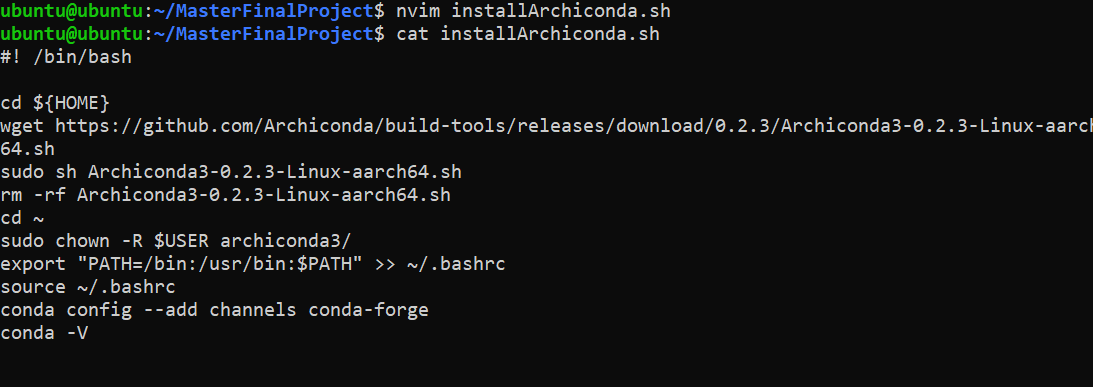
\includegraphics[scale=0.7]{fig/installArchiconda.PNG}
    \caption{Creación archivo instalador archiconda.}
    \label{fig:mesh1}
\end{figure}

\begin{figure}[h]
    \centering
    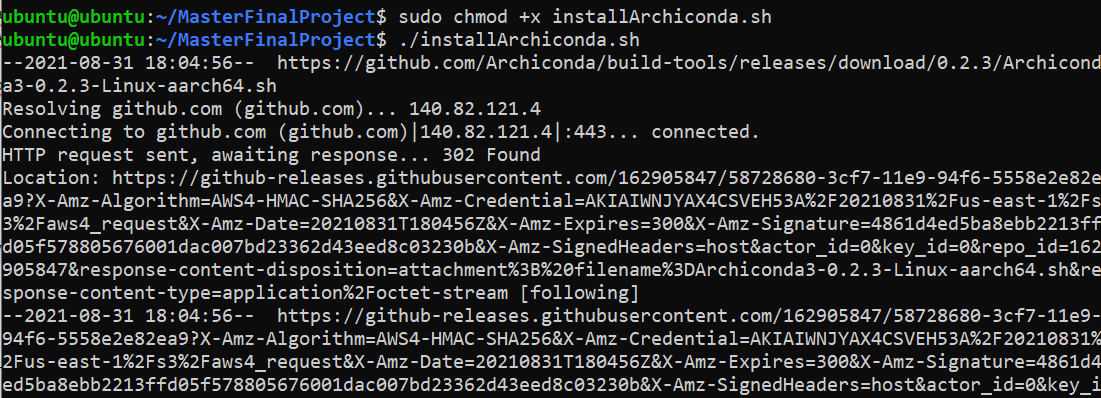
\includegraphics[scale=0.7]{fig/archicondaInstalling.PNG}
    \caption{Ejecución archivo instalador archiconda.}
    \label{fig:mesh1}
\end{figure}

Una vez se ha instalado archiconda, se puede comprobar que se ha instaladao corerrectamente ejecutando el comando " conda --version " o bien " conda -V ". Si este comando devuelve la versión de conda significará que se ha isntalado correctamente y estará todo listo para crear un entorno e instalar los diferentes paquetes necesarios.

Con el gestor de paquetes conda se puede proceder a la instalación y preparación de todo el entorno de desarrollo. El primer de los pasos a seguir para poder poner a punto el proyecto, es crear un entorno aislado donde poder compilar y donde poder alojar todos los paquetes necesarios para que a la hora de ejecutar se puedan encontrar todas las librerías en el entorno adecuado. Para poder hacer esto el primero de los comando a ejecutar es " conda create --name tflite1-env ".
 
 \begin{figure}[h]
    \centering
    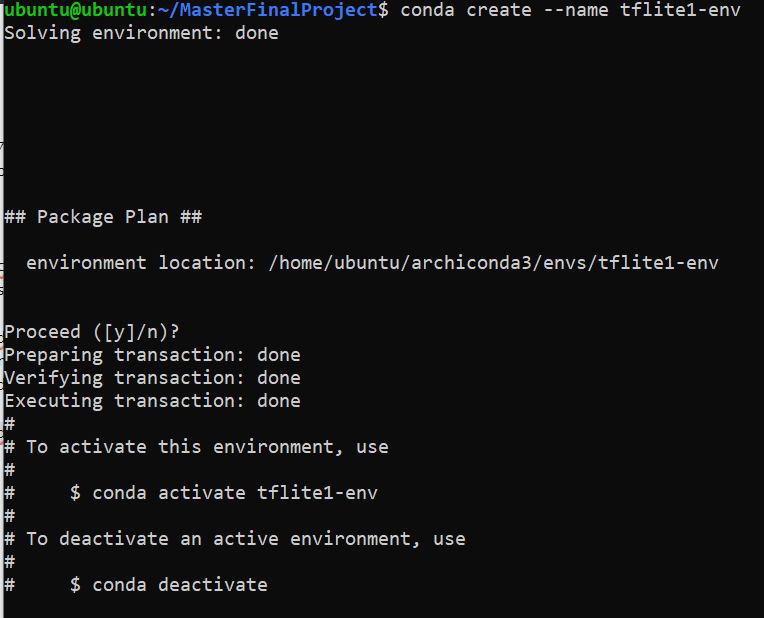
\includegraphics[scale=0.7]{fig/conda create.PNG}
    \caption{Ejecución archivo instalador archiconda.}
    \label{fig:mesh1}
\end{figure}

Una vez creado el entorno conda donde poder ejecutar los comandos, el siguiente paso será poder ejecutar " conda activate tflite1-env ". De esta forma se activa el entorno conda donde se quiere trabajar y estará todo preparado para poder empezar a instalar dependencias.

\begin{figure}[h]
    \centering
    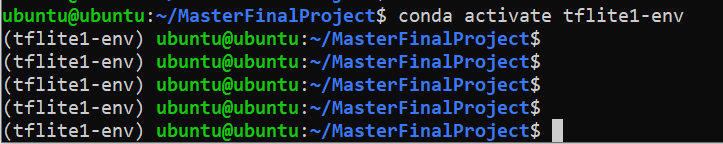
\includegraphics[scale=0.7]{fig/conda activate.PNG}
    \caption{Ejecución archivo instalador archiconda.}
    \label{fig:mesh1}
\end{figure}

El siguiente paso es instalar las dependencias, para poder instalar las dependencias desde un mismo scripts se han seguido los mismos pasos que se han seguido para la instalación de archiconda. Los requerimientos para poder ejecutar la detección de objetos vienen en el siguiente archivo ejecutable:

\begin{lstlisting}[language=bash, caption={Código bash}, label={cod:bash}, captionpos=b]
#!/bin/bash

# Get packages required for OpenCV

sudo apt-get -y install libjpeg-dev libtiff5-dev libjasper-dev libpng12-dev
sudo apt-get -y install libavcodec-dev libavformat-dev libswscale-dev libv4l-dev
sudo apt-get -y install libxvidcore-dev libx264-dev
sudo apt-get -y install qt4-dev-tools libatlas-base-dev

# Need to get an older version of OpenCV because version 4 has errors
pip3 install opencv-python
# pip install opencv-python (If pip3 drops you an error)

# Get packages required for TensorFlow
# Using the tflite_runtime packages available at https://www.tensorflow.org/lite/guide/python
# Will change to just 'pip3 install tensorflow' once newer versions of TF are added to piwheels

#pip3 install tensorflow
# Modded for installin tflite on a RPI4 running ubuntu mate 20.04
version=$(python -c 'import sys; print(".".join(map(str, sys.version_info[:2])))')

if [ $version == "3.7" ]; then
pip3 install --extra-index-url https://google-coral.github.io/py-repo/ tflite_runtime
fi

if [ $version == "3.5" ]; then
pip3 install --extra-index-url https://google-coral.github.io/py-repo/ tflite_runtime
fi
\end{lstlisting}

Una vez instalado el fichero de requierements, la raspberry estará lista para poder ejecutar una red neuronal precompilada. El siguiente de los pasos consiste en poder establecer la Coral TPU como dispositivo que será encargado de poder procesar toda esta información y poder realizar la detección de objetos.

En este punto la Raspberry es capaz de compilar y poder ejecutar la detección de objetos. Esto se puede conseguir tanto desde una entrada de vídeo como puede ser por ejemplo una webcam, o bien se puede conseguir procesar una imagen o vídeo y aplicar los coeficientes de la red neurona para poder clasificar los diferentes inputs que puedan llegar a través del vídeo. 


\subsection{Comunicación entre dispositivos}

Con el objetivo de poder establecer la comunicación entre todos los dispositivos que formarán parte del robot final, se ha decidido establecer una comunicación serie a través de una UART. 


\subsection{Scripts de python}

\subsection{Imagen Linux}